\section{Results}
To demonstrate \deploy's capability to effectively conduct transition
scenario analysis and meet the objectives described in section 
\ref{sec:obj}, this section will 
(1) demonstrate \deploy's capability in simple transition scenarios, 
(2) compare the prediction methods for different transition scenarios, and
(3) demonstrate using \deploy to set up successful EG01-EG23, EG01-EG24, 
EG01-EG29, and EG01-EG30 transition scenarios. 
The input files and scripts to produce the results and plots in this
paper can be reproduced using \cite{dnoauthor_d3ploy:_2018}, and 
\cite{chee_arfc/transition-scenarios_2018}. 

\subsection{Demonstration of \deploy's capabilities}
\label{sec:demo}
A simple linearly increasing power demand simulation is conducted 
to demonstrate \deploy's capabilities for 
simulating transition scenarios and to inform decisions about 
input parameters when setting up larger transition scenarios 
with many facilities.
This simulation is a simple transition scenario that only include 
three types of facilities: \texttt{source}, \texttt{reactor}, and 
\texttt{sink}. 
The simulation initially has ten initial \texttt{reactor} facilities 
(\texttt{reactor1} to \texttt{reactor10}). 
These reactors have staggered cycle lengths and lifetimes to prevent 
simultaneous refueling and set up gradual decommissioning. 
\deploy is set up to deploy \texttt{new reactor} facilities
to meet the loss of power supply introduced from the decommissioning 
of the initial \texttt{reactor} facilities. 
The \deploy input parameters for the simulation is shown in Table 
\ref{tab:demonstrations}. 

    \begin{table}[]
        \resizebox{\textwidth}{!}{%
        \caption{\deploy's input parameters for the simple transition scenarios.}
        \label{tab:demonstrations}
        \begin{tabular}{l|l|l}
        \hline
                                  & \textbf{Input Parameters}          & \textbf{Simple Transition Scenario: Linearly Increasing Power} \\ \hline
        \multirow{5}{*}{R\textbf{equired}} & Demand driving commodity  & \multicolumn{1}{l}{Power}                            \\
                                  & Demand equation [MW]          &  $t<40 = 1000, t\geq 40 = 250t$                                                    \\
                                  & Facilities it controls    &  \texttt{Source}, \texttt{Reactor}, \texttt{Sink}                                                    \\
                                  & Prediction method         &  \texttt{FFT}                                                    \\
                                  & Deployment driving method & \multicolumn{1}{l}{Installed Capacity}               \\ \hline
        \multirow{2}{*}{\textbf{Optional}} & Buffer type               & \multicolumn{1}{l}{Absolute}                         \\
                                  & Buffer size               &  Power: 2000MW, Fuel: 1000kg                                                    \\ \hline
        \end{tabular}%
        }
        \end{table}

Figures \ref{fig:growingtransition-power}, \ref{fig:growingtransition-fuel}
and \ref{fig:growingtransition-spentfuel} demonstrate \deploy's capability 
to deploy reactor and supporting facilities to meet the linearly increasing
power demand and subsequently demanded secondary commodities with 
minimal undersupply.
Figure \ref{fig:growingtransition-power} demonstrates that
the main objective of \deploy was met since there are no timesteps
in which the supply of power falls under demand.
By using a combination of the \texttt{FFT} method for 
predicting demand and setting the supply buffer to 2000MW 
(the capacity of 2 reactors), the user minimizes the number of 
undersupplied timesteps for every commodity.

In figure \ref{fig:growingtransition-fuel},
a facility with a large fuel throughput is initially
deployed to meet the large initial fuel demand for the starting
up of ten reactors. 
\deploy is prevented from deploying many supporting
facilities that end up being redundant at the later parts of 
the simulation, by having an initial facility with a large throughput
exist for the first few timesteps in the simulation.
This is a reflection of reality in which reactor manufacturers will 
accumulate an appropriate amount of fuel inventory before starting 
up reactors. 
There is one timestep where there is an undersupply after the 
decommissioning of the large initial facility.  
This is unavoidable since the prediction methods in \deploy are 
unable to predict this sudden drop in demand. 

\begin{figure}[]
    \centering
    \begin{subfigure}[t]{\textwidth}
    \centering
        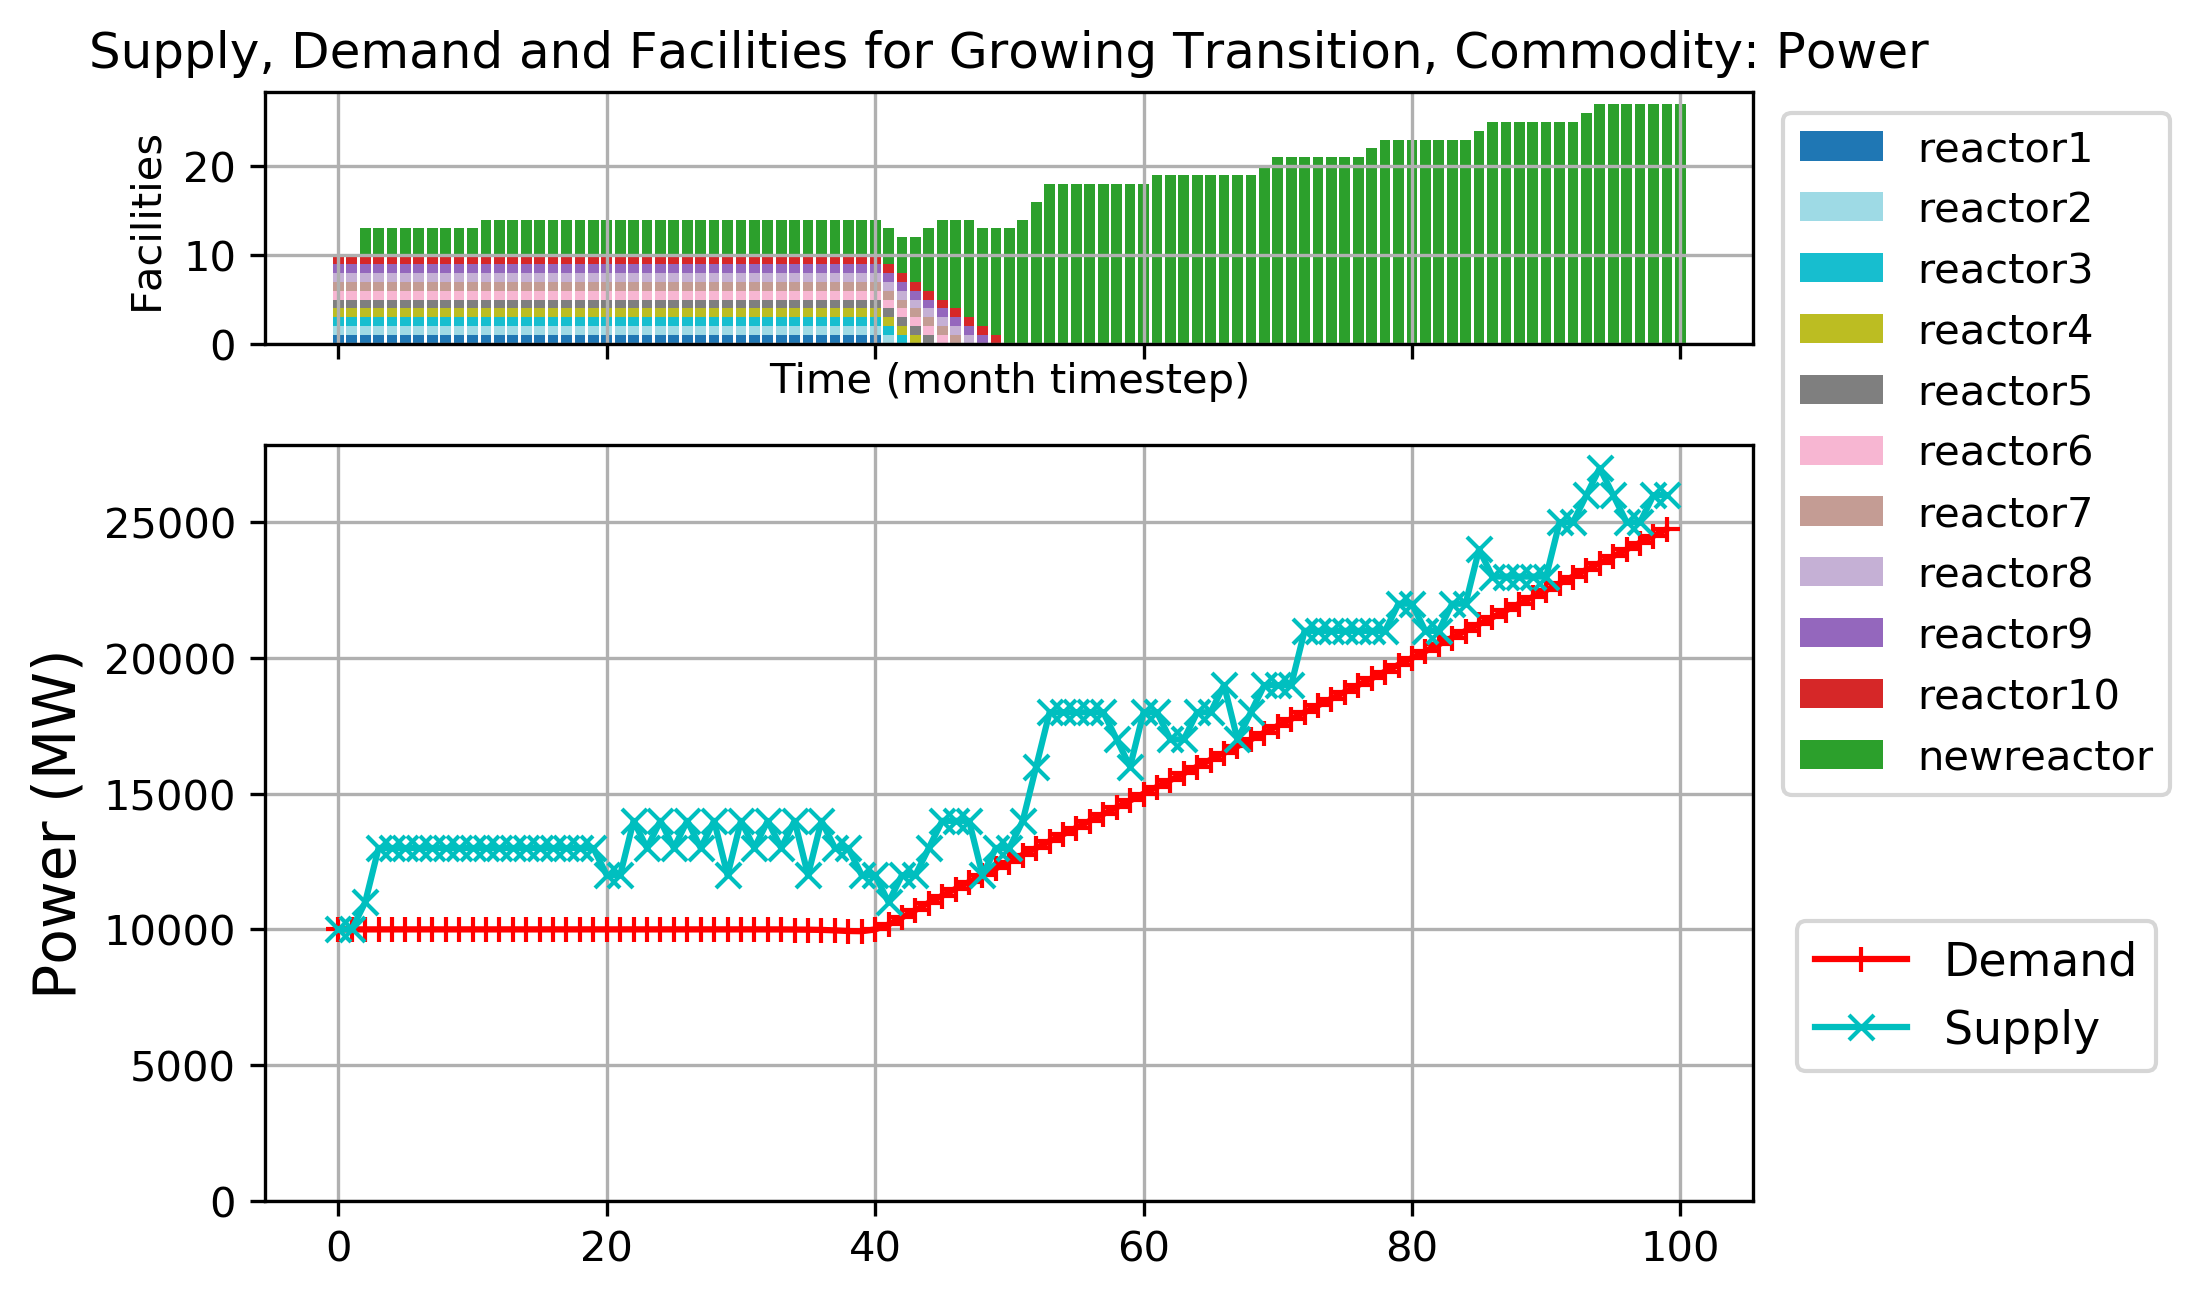
\includegraphics[width=0.8\linewidth]{figures/growingtransition-power.png} 
        \caption{The power demand is a user-defined equation and power is supplied by the reactors.
        There are no time steps with undersupply of power.}
        \label{fig:growingtransition-power}
    \end{subfigure}
    \begin{subfigure}[t]{0.65\textwidth}
        \centering
        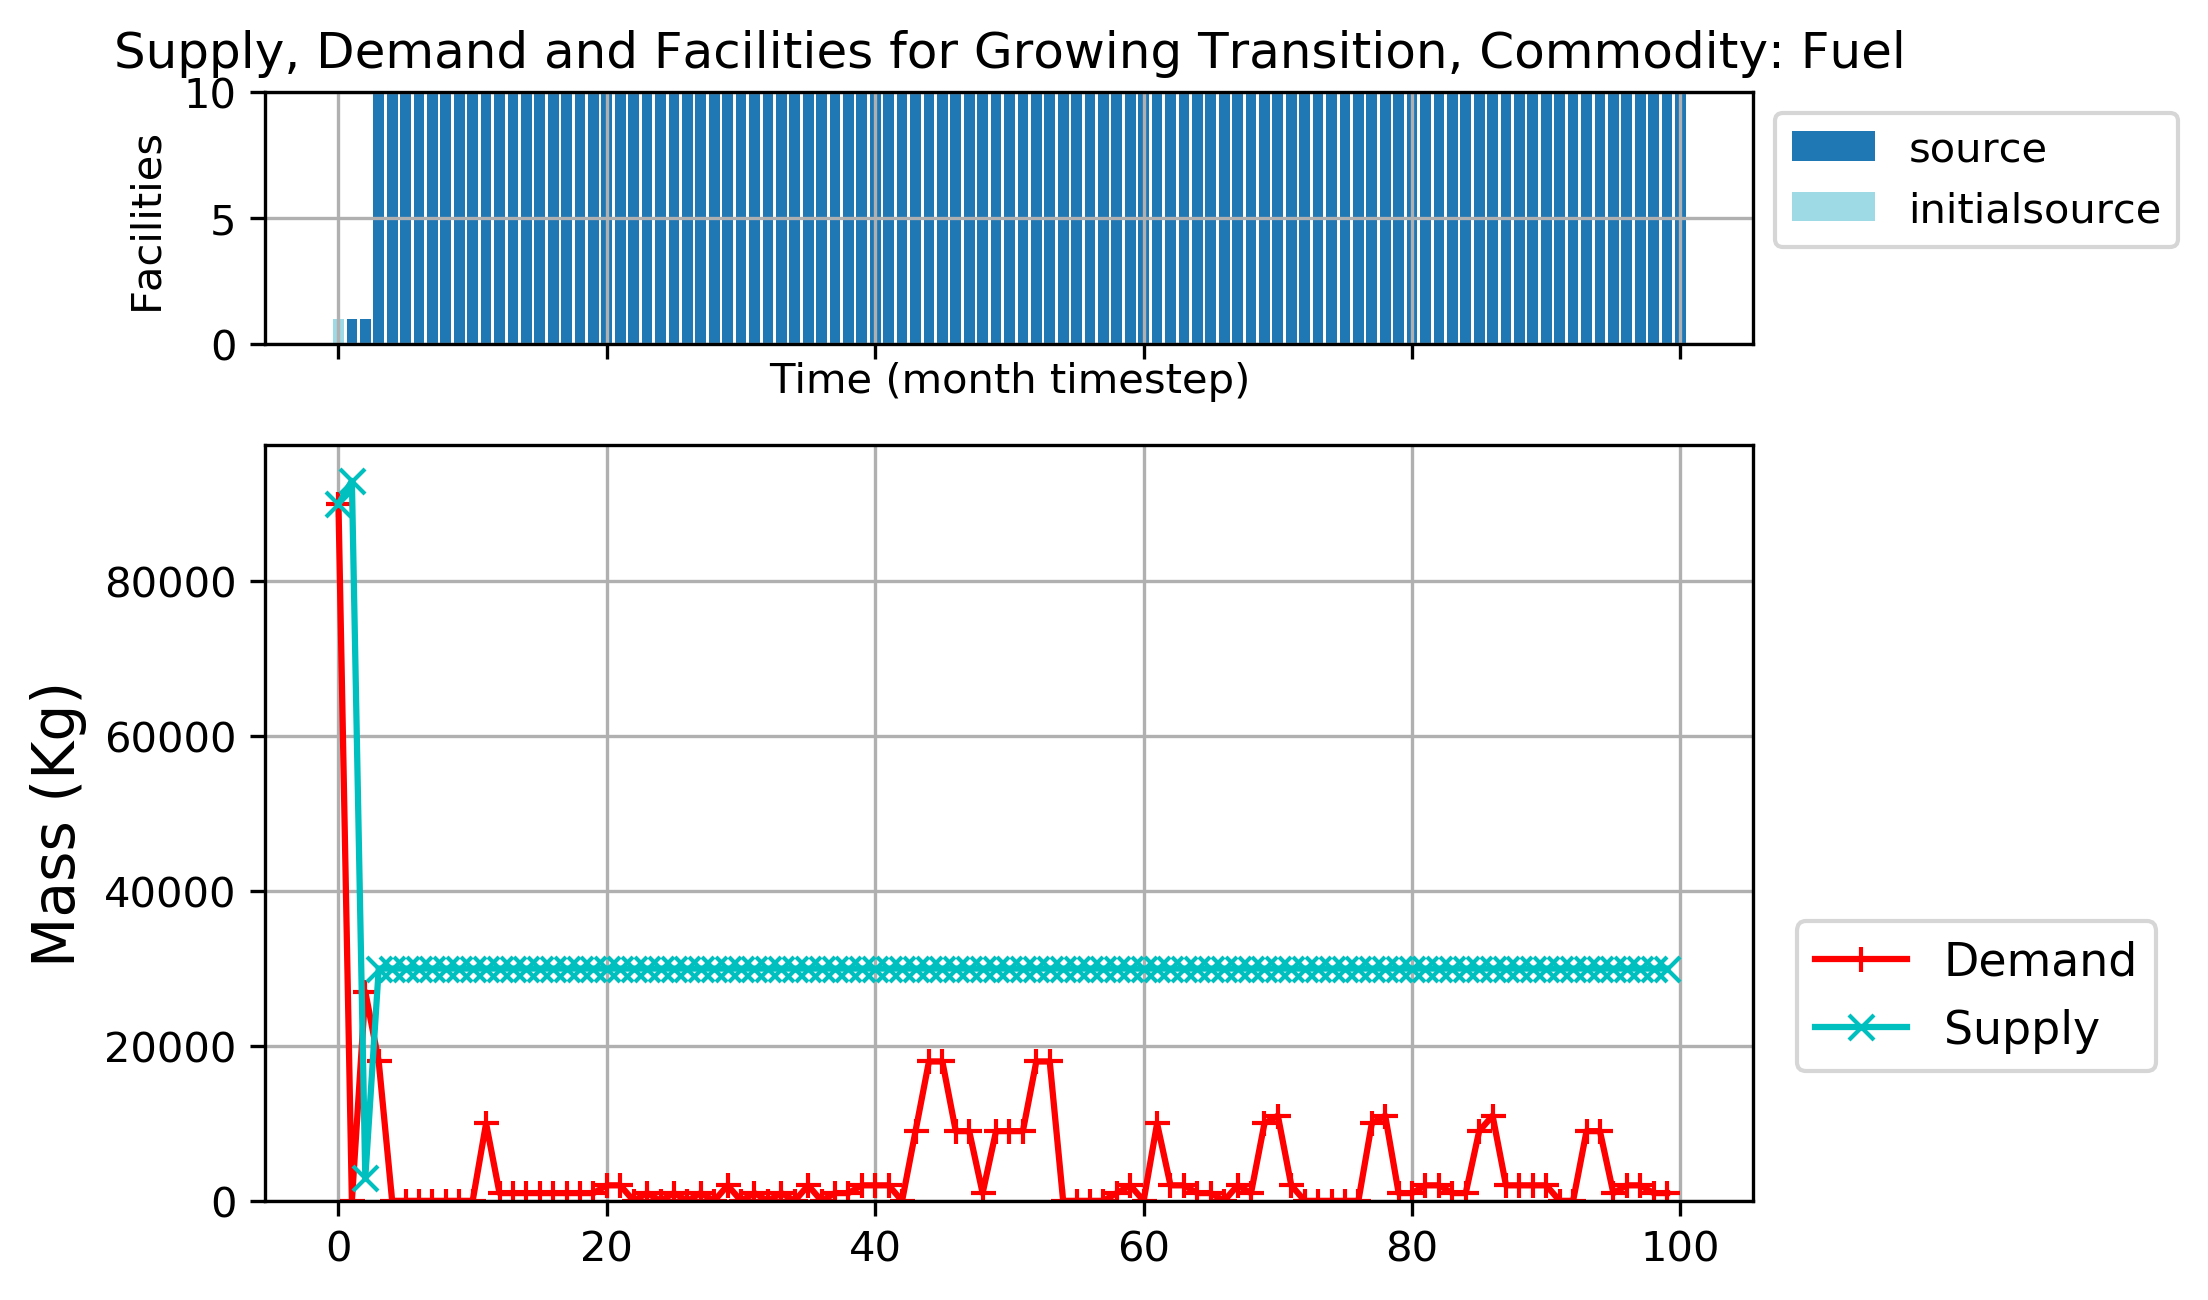
\includegraphics[width=\linewidth]{figures/growingtransition-fuel.png} 
        \caption{Fuel is demanded by reactors and supplied by source facilities.
        There are is only one time step with undersupply of fuel.}
	    \label{fig:growingtransition-fuel}
    \end{subfigure}
    \begin{subfigure}[t]{0.65\textwidth}
        \centering
        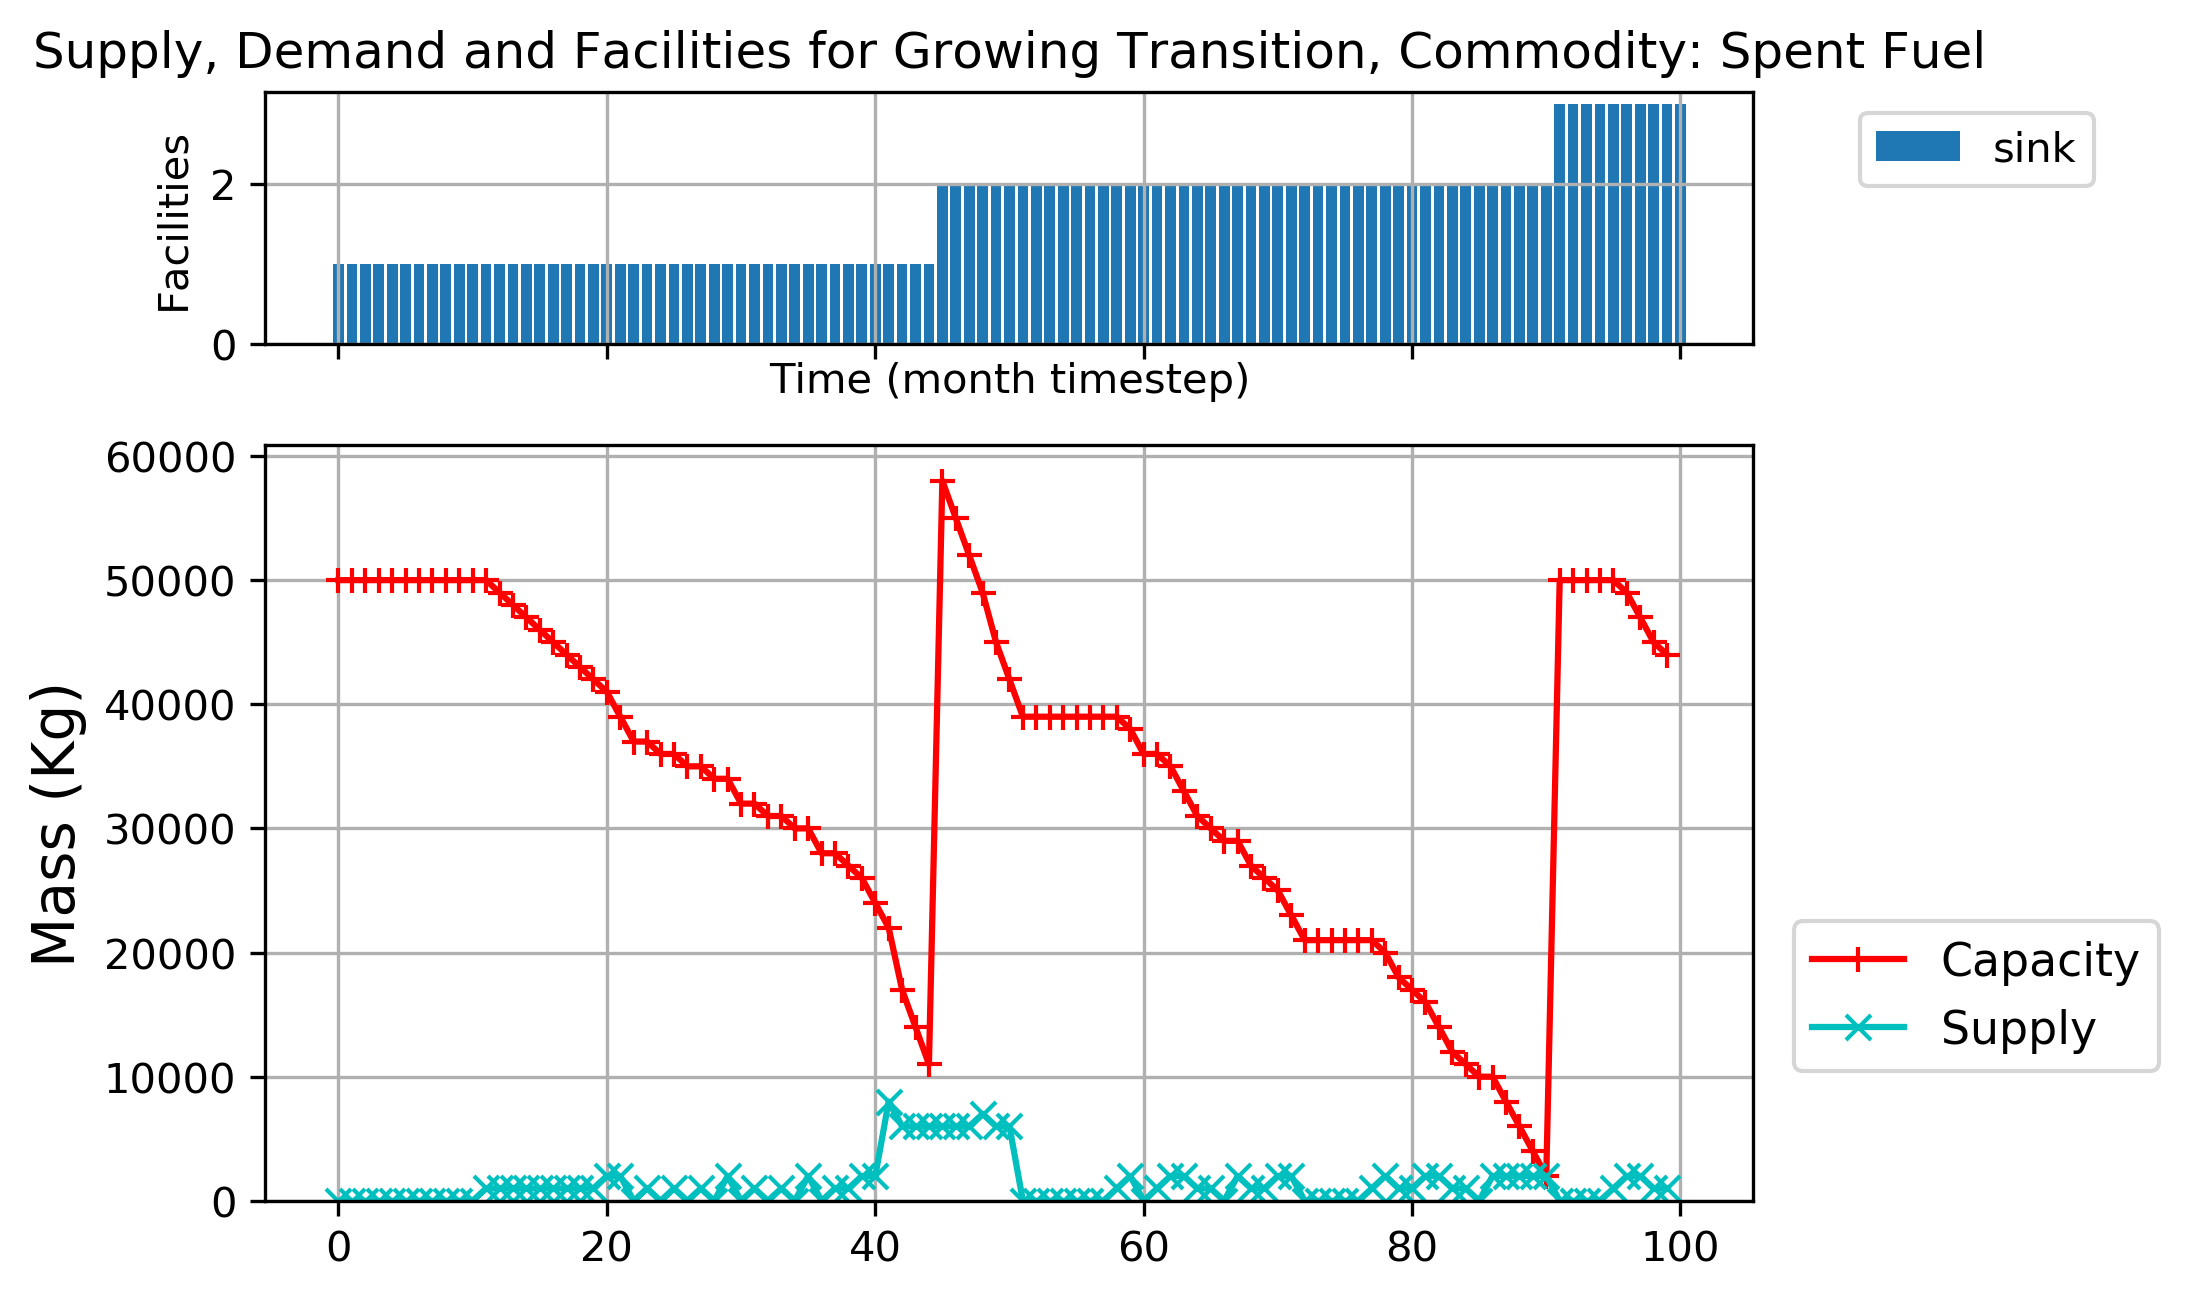
\includegraphics[width=\linewidth]{figures/growingtransition-spentfuel.png} 
        \caption{Spent Fuel is supplied by reactors and the capacity is provided by sink facilities.
        There are no time steps with under capacity of sink space.}
        \label{fig:growingtransition-spentfuel}
    \end{subfigure}
    \caption{Transition Scenario: Linearly increasing power demand.}
\end{figure}
